% 2_5_lqr_design.tex
% !TeX root=../main.tex

\section{طراحی کنترل‌کننده خطی درجه دوم (\lr{LQR})}
\label{sec:lqr_design}

به‌منظور پایدارسازی سیستم حول نقطه تعادل و بررسی عملکرد آن در حلقه بسته، کنترل‌کننده فیدبک حالت بهینه از نوع خطی درجه دوم (\lr{LQR}) مورد ارزیابی قرار می‌گیرد. همان‌طور که در بخش‌های پیشین اثبات شد، مکانیزم تغییر طول کابل در تقریب خطی فاقد اثرگذاری دینامیکی مستقیم است. بر این اساس، در این بخش طول کابل ثابت فرض شده ($l = l_0 = 0.5$ متر) و مکانیزم وینچ غیرفعال در نظر گرفته می‌شود ($\dot{l} = 0$ و $\ddot{l} = 0$). در نتیجه، تنها عملگر فعال سیستم نیروی محرک ارابه ($F$) است و ماتریس توزیع ورودی ($B_{LQR}$) به ستون اول ماتریس $B$ تقلیل می‌یابد:
\begin{equation}
    B_{LQR} = \begin{bmatrix} 0 \\ \frac{1}{M} \\ 0 \\ -\frac{1}{M l_0} \end{bmatrix}
\end{equation}

تئوری کنترل \lr{LQR} بر پایه حداقل‌سازی یک تابع هزینه در افق بی‌نهایت (\lr{Infinite Horizon}) به فرم درجه دوم بنا شده است. این تابع هزینه تعادلی میان خطای حالت (انحراف از نقطه تعادل) و تلاش کنترلی (انرژی مصرفی عملگرها) ایجاد می‌کند:
\begin{equation}
    J = \int_{0}^{\infty} \left( x^T Q x + u^T R u \right) dt
\end{equation}
که در آن $x$ بردار حالت سیستم، $u$ سیگنال کنترلی (نیروی $F$)، $Q$ ماتریس نیمه‌معین مثبت وزن حالات و $R$ پارامتر معین مثبت وزن ورودی است. با توجه به مقادیر فیزیکی سیستم ($M = 1$، $m = 0.2$، $g = 9.81$، $b_c = 0.1$ و $b_p = 0.05$)، ماتریس‌های وزن بر اساس اهمیت متغیرهای کنترلی به صورت زیر تنظیم شده‌اند:
\begin{equation}
    Q = \text{diag}([1000, 10, 500, 10])
\end{equation}
\begin{equation}
    R = 1
\end{equation}

درایه $Q_{11} = 1000$ نشان‌دهنده جریمه سنگین بر خطای موقعیت کالسکه ($x$) است تا سیستم با سرعت بالایی به نقطه هدف همگرا شود. همچنین درایه $Q_{33} = 500$ به‌منظور اعمال قید نرم بر زاویه آونگ ($\theta$) و سرکوب نوسانات انتخاب شده است. انتخاب $R = 1$ نیز اجازه می‌دهد تا کنترل‌کننده از ظرفیت عملگر نیرو به نحو مطلوب بهره‌برداری کند.

قانون کنترل بهینه به فرم فیدبک حالت $u = -Kx$ تعریف می‌شود. ماتریس بهره فیدبک ($K$) از طریق حل معادله جبری ریکاتی (\lr{Algebraic Riccati Equation}) به دست می‌آید:
\begin{equation}
    A^T P + P A - P B_{LQR} R^{-1} B_{LQR}^T P + Q = 0
\end{equation}
\begin{equation}
    K = R^{-1} B_{LQR}^T P
\end{equation}

برای محاسبه ماتریس بهره بهینه $K$، از توابع استاندارد نرم‌افزار متلب استفاده شده است (جزئیات و کدهای راه‌اندازی این بخش در قالب برنامه \ref{code:lqr_init} در پیوست \ref{app:matlab_codes} ارائه شده است). با حل این معادله، ماتریس بهره برای سیستم مورد مطالعه به صورت زیر استخراج می‌شود:
\begin{equation}
    K = \begin{bmatrix} 31.6228 & 14.0488 & -17.7264 & 0.3611 \end{bmatrix}
\end{equation}

سیگنال کنترلی نهایی تولید شده توسط این استراتژی برابر با $F = -Kx$ است. معماری حلقه بسته این کنترل‌کننده در محیط شبیه‌سازی در شکل \ref{fig:lqr_block_diagram} نشان داده شده است. با توجه به این دیاگرام، ورودی شتاب کابل ($\ddot{l}$) با مقدار ثابت $0$ تغذیه شده است که پس از دو مرحله انتگرال‌گیری پیوسته، طول کابل را در مقدار اولیه خود قفل می‌کند. همزمان، بردار حالت سیستم از محیط فیزیکی استخراج شده و پس از ضرب در ماتریس بهره ($-K$)، فرمان کنترلی فیدبک برای اعمال نیروی کالسکه را شکل می‌دهد. این ساختار مدار بسته، برای ارزیابی عملکرد سیستم در مواجهه با شرایط اولیه و خطاهای موقعیت مختلف در ادامه پژوهش مورد تحلیل قرار می‌گیرد.

\begin{figure}[ht]
    \centering
    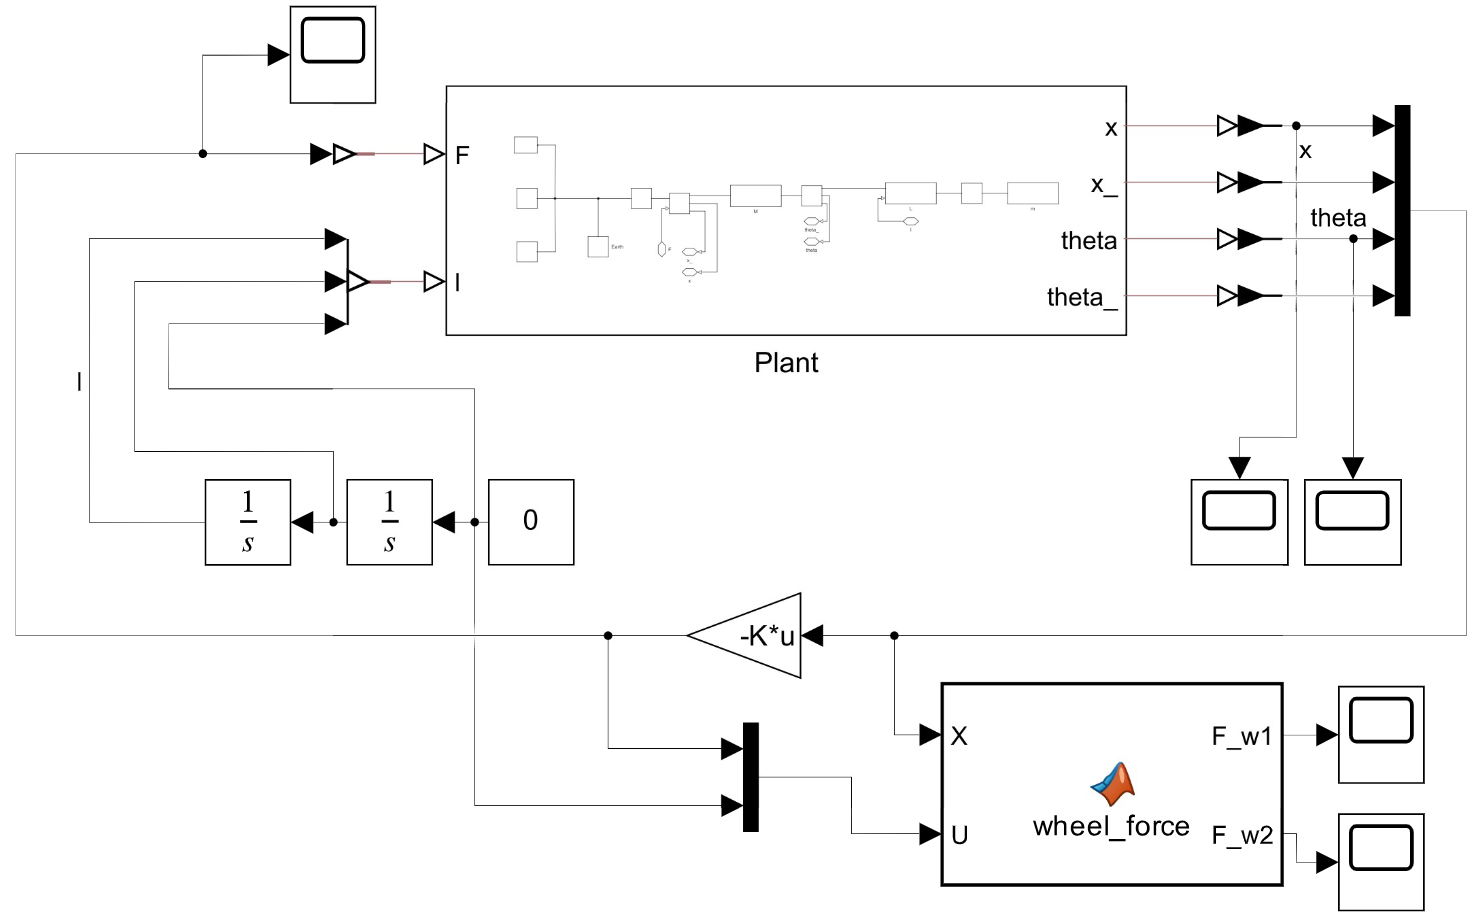
\includegraphics[width=\textwidth]{images/1_LQR_Step/LQR_block_diagram.png}
    \caption{\rl{معماری حلقه بسته کنترل‌کننده خطی \lr{LQR} با فرض طول کابل ثابت}}
    \label{fig:lqr_block_diagram}
\end{figure}